% This is samplepaper.tex, a sample chapter demonstrating the
% LLNCS macro package for Springer Computer Science proceedings;
% Version 2.20 of 2017/10/04
%
\documentclass[runningheads]{llncs}
%
\usepackage{graphicx}
\usepackage{amssymb}
\usepackage{amsmath}
\usepackage{hyperref}
\usepackage{tikz}
\usetikzlibrary{matrix}
\usepackage[toc,page]{appendix}

% Used for displaying a sample figure. If possible, figure files should
% be included in EPS format.
%
% If you use the hyperref package, please uncomment the following line
% to display URLs in blue roman font according to Springer's eBook style:
% \renewcommand\UrlFont{\color{blue}\rmfamily}

\begin{document}
%
\title{An Evaluation of Uninformed and Informed Search Algorithms on the k-puzzle Problem\thanks{Supported by Prof Yair Zick and Prof Daren Ler.}}
%
\titlerunning{Evaluation of Search Algos on k-puzzle}
% If the paper title is too long for the running head, you can set
% an abbreviated paper title here
%
\author{Dalis Chan \textit{(A0187451Y)} \and
Johanna \textit{(A0187536R)} \and
Sean Low Chen Yi \textit{(A0183743Y)} \and 
Law Ann Liat, Larry \textit{(A0189883A)}}
%
% First names are abbreviated in the running head.
% If there are more than two authors, 'et al.' is used.
%

\institute{National University of Singapore \\
Repository Link \href{https://github.com/larrylawl/CS3243-project-1}{here}}
%
\maketitle              % typeset the header of the contribution
%
\begin{abstract}
K-puzzle is often used as test problems for new search algorithms in artificial intelligence ~\cite[p71]{stuart_russell_artifical_2010}. This paper evaluates the use of iterative deepening search (IDS) and \( A^* \) search. 
Since \( A^* \) search uses heuristic functions to guide its search, this paper also evalutes the heuristic functions euclidean distance, manhattan distance, and linear conflict.
\end{abstract}
%
%
%
\section{Problem Specification}
\begin{enumerate}
    \item \textbf{State:} For \( k \in \{3, 4, 5\} \),  a \( k \times k \) matrix \( M \) with each entry \( m_{i, j} \) being a unique integer from \( \{0, 1, \cdots, 8 \} \) where 0 represents the blank tile.
    \item \textbf{Initial State:} Puzzle can start in any state \textit{s}.
    \item \textbf{Actions or \textit{Actions(s)}:} Let \( m_{k, l} \in M \) denote the blank tile and \( m_{i, j} \in M \) denote the tile \textbf{adjacent} to the blank tile \( m_{k, l} \).
    Actions are movements of the adjacent tile \( m_{i, j} \) towards the blank tile \( m_{k, l} \). For example, the action \textit{Left} moves the adjacent tile \( m_{k, l+1} \in M \) to the blank tile \( m_{k, l} \).
    \item \textbf{Transition Model or \textit{Result(s,a)}:} \( Result(s, a) \) swaps the pair of tiles specified in action \( a \) in the current state \textit{s} and returns this new state \textit{s'}.
    \item \textbf{Goal State:}
    \[
    M_{goal}= \begin{bmatrix}
        1 & 2 & 3 \\
        4 & 5 & 6 \\
        7 & 8 & 0
        \end{bmatrix}
    \]
    \item \textbf{Path Cost:} Every step cost \textit{c(s, a, s') = 1}, and the path cost is the summation of the step costs from the initial state to the goal state.
\end{enumerate}

\section{Technical Analysis of the Selected Algorithms and Heuristics}

\subsection{Rule to Check if k-puzzle is Solvable}
\textbf{Definition.} A pair of tiles form an \textit{inversion} if the values on tiles are in the reverse order of their appearance in the goal state. \\
\textbf{Rules~\cite{aditya_goel_how_nodate}.} Let \( M \) denote a \( k \times k \) matrix, \( m_{i, j} \) denote a blank tile in \( M \), and \( n_i \) denote the number of inversions in the intial state \( M_{initial} \). Puzzle is solvable if \dots
\begin{enumerate}
    \item \( k \) is odd and \( n_i \) is even
    \item \( k \) is even,
    \begin{enumerate}
        \item \( n_i \) is odd and \( m_{i,j} \) is on an even row from the bottom (ie \( j \) is odd).
        \item \( n_i \) is even and \( m_{i,j} \) is on an odd row from the bottom (ie \( j \) is even).
    \end{enumerate}
\end{enumerate}

\subsection{Uninformed Search}
\begin{enumerate}
    \item \textbf{Implementation:} Graph-based IDS. Step costs are equal, thus it is optimal. Furthermore, since the search space is large and the depth of the solution is not known, IDS is preferred ~\cite[p90]{stuart_russell_artifical_2010}.
    \item \textbf{Correctness:} Branching factor \( b = 4 \) is finite, thus IDS is complete ~\cite[p88-90]{stuart_russell_artifical_2010}. 
    \item \textbf{Time Complexity:} \( O(b^d) \) ~\cite[p88-90]{stuart_russell_artifical_2010}.
    \item \textbf{Space Complexity:} \( O(bd) \) ~\cite[p88-90]{stuart_russell_artifical_2010}.
\end{enumerate}

% TODO Add in proofs for heuristic
\subsection{Informed Search}
\begin{enumerate}
    \item \textbf{Implementation:} Graph-based \( A^* \) search. It improofs on greedy best first search (ie \( f(n) = h(n) \)) as it avoids expanding paths that are already expensive (ie \( f(n) = g(n) + h(n) \)).
    \item \textbf{Correctness:} Since the search space is finite, \( A^* \) search will be complete.
    \item \textbf{Time Complexity:} \( O(b^{h^*(s_0) - h(s_0)}) \) ~\cite[p93-99]{stuart_russell_artifical_2010}.
    \item \textbf{Space Complexity:} \( O(b^m) \) ~\cite[p93-99]{stuart_russell_artifical_2010}.
\end{enumerate}

\subsection{\(h_1:\) Euclidean Distance}
\textbf{Definition.} Euclidean Distance heuristic is defined as the straight line distance between the tiles from their goal position ~\cite{rosalind_euclidean_nodate}. \\
\textbf{Proof for Consistency.} Euclidian distance is a form general triangle inequality, given that the euclidian distance from start state \( S \) to end state \( G \) (1 side of the triangle) cannot be longer than the sum of the 2 sides ( the actual distance from S to middle state N and the euclidian distance from N to G) as the euclidian distance from \( S \) to \( G \) is already the shortest path. 
Since general triangle inequality fulfills the definition of consistency ~\cite[p95]{stuart_russell_artifical_2010}, euclidean distance is consistent.

\subsection{\(h_2:\) Manhattan Distance} 
\textbf{Definition.} Manhattan Distance heuristic is defined as the sum of the distance of the tiles from their goal positions ~\cite[p103]{stuart_russell_artifical_2010} . Note that this sum only includes horizontal and vertical distances as \textit{Actions} do not allow the diagonal movements. \\
\textbf{Proof for Consistency.} Proof for consistency can be found in appendix \ref{appendix:manhat_cons}.

\subsection{ \(h_3: \) Linear Conflict}
\textbf{Definition.} Two tiles \( t_j \) and \( t_k \) are in a linear conflict if \( t_j \) and \( t_k \) are in the same line, 
the goal positions of \( t_j \) and \( t_k \) are both in that line, 
\( t_j \) is to the right of \( t_k \), and the goal position of \( t_j \) is to the left of the goal position of \( t_k \) \cite[p13]{othar_hansson_generating_1985}. \\
\textbf{Derivation.} For any state \( s \),
\begin{enumerate}
    \item For each tile \( t_j \) in \( r_i \), let \( C(t_j, r_i) \) denote the number of tiles conflicting with \( t_j \) in row \( r_i \).
    \item While there is a non-zero \( C(t_j, r_i) \) value,
    \begin{enumerate}
        \item Move out the tile with the most conflicts from \( r_i \). Let this tile be \( t_k \).
        \item Set \( C(t_k, r_i) \) = 0.
        \item For every tile \( t_j \) in conflict with \( t_k \), decrement \( C(t_j, r_i) \) by 1.
        \item Let \( lc(s, r_i) \) denote the number of tiles that must be removed from row \( r_i \) in order to resolve the linear conflicts in \( r_i \). Increment \( lc(s, r_i) \) by 1.
    \end{enumerate}
    \item Repeat Step 1 and 2 for other rows and columns and sum the values of all \( lc (s, r_i) \) and \( lc(s, c_i) \).
    \item Let \( LinearConflict(s) \) denote the minimum number of additional moves necessary to resolve the linear conflicts in state \( s \). \( LinearConflict(s) \) = 2 x result from Step 3.
    \[
        h_3(s) = ManhattanDistance(s) + LinearConflict(s)
    \]
\end{enumerate}
\textbf{Prove for Consistency.} To prove consistency, we must prove that for all \( s \) and \( s' \), \( f(s') \geq f(s) \), where \( s' \) is the successor of \( s \).
\[
    f(s) = g(s) + h(s)
\]
, where $g(s') = g(s) + 1$ and $h(s) = ManhattanDistance(s) + LinearConflict(s)$. \\
Assume that tile \( t_k \) moves from row \( r_i \) to row \( r_j \) and stays in the same column. Let \( ManhattanDistance(s) \) be \( MD(s) \) and \( LinearConflict(s) \) be \( LC(s) \). 
\begin{enumerate}
    \item \textbf{Condition 1:} Both \( r_i \) and \( r_j \) are not the goal row of \( t_j \).
    
        \( MD(s') = MD(s) \pm 1 \). \( LC(s) \) is unchanged. Thus, \( h(s') = h(s) \pm 1 \) and \( f(s') = f(s) + 1 \pm 1 \geq f(s) \).
    
    \item \textbf{Condition 2:} \( r_j \) is the goal row of \( t_j \).
        
        As \( t_j \) moves to its goal row, \( MD(s') = MD(s) - 1 \). Since \( r_i \) is not the goal row of \( t_j \), \( lc(s', r_i) = lc(s, r_i) \). 
        As \( r_j \) is the goal row, the conflicts in row \( r_j \) may or may not increase; so it is either \( lc(s', r_j) = lc(s, r_j) \) or \( lc(s', r_j) = lc(s, r_j) + 2 \). 
        Hence, \( h(s') = h(s) \pm 1 \) and \( f(s') = f(s) + 1 \pm 1 \geq f(s) \).

    \item \textbf{Condition 3:} \( r_i \) is the goal row of \( t_j \).
    
        As \( t_j \) moves away from its goal row, \( MD(s') = MD(s) + 1 \). 
        As \( r_i \) is the goal row, the conflicts in row \( r_i \) may or may not decrease; so it is either \( lc(s', r_i) = lc(s, r_i) \) or \( lc(s', r_i) = lc(s, r_i) + 2 \). 
        Since \( r_j \) is not the goal row of \( t_j \), \( lc(s', r_j) = lc(s, r_j) \). 
        Therefore, \( h(s') = h(s) \pm 1 \) and \( f(s') = f(s) + 1 \pm 1 \geq f(s) \).
\end{enumerate}
All 3 cases show that \( f(s') \geq f(s) \). Thus, for any tile which moves from column \( c_i \) to \( c_j \) while remaining in the same column, \( f(s') \geq f(s) \) will still hold by the symmetry of the puzzle.


\section{Experimental Setup}
\subsection{Description}
The three informed searches were tested against 3 x 3 puzzles of varying difficulty and their runtimes are plotted against the number of nodes it passed to achieve goal states. To minimize bias, the searches were tested against 30 different puzzles for each number of steps needed to achieve goal states and the average of the 30 values of nodes passed are taken. See
Fig.~\ref{fig1} for the visualization of the results.

\begin{figure}
    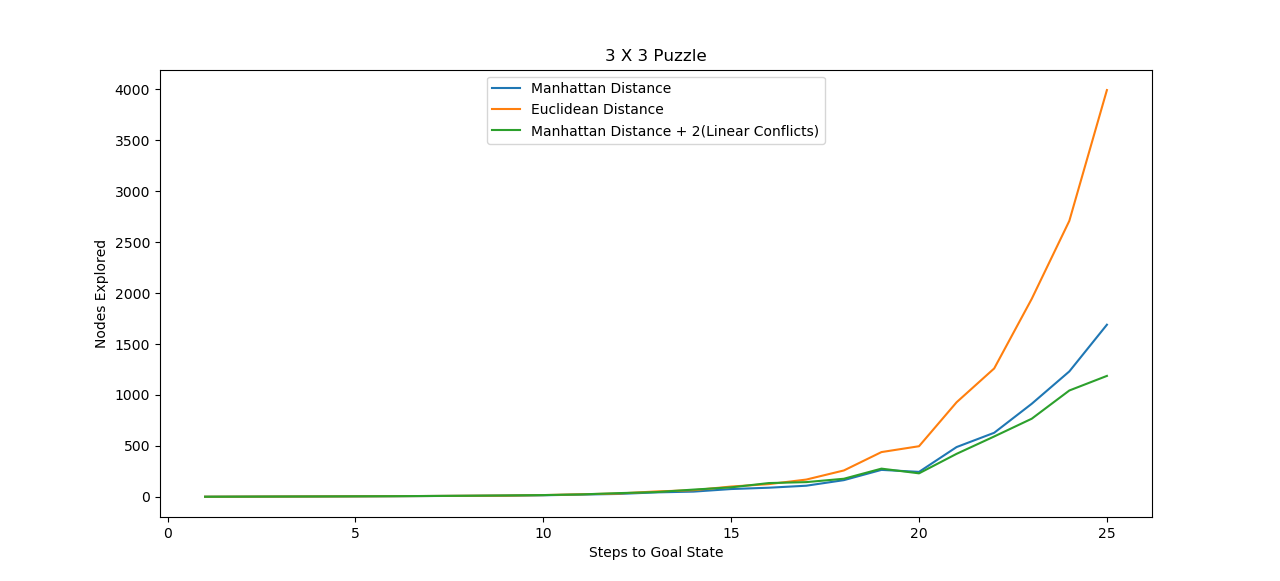
\includegraphics[width=\textwidth]{fig1.png}
    \caption{Performance of the three different heuristics under varying levels of k-puzzle difficulty.} \label{fig1}
    \end{figure}

\subsection{Analysis}
For simple problems (number of steps is less than 15), the differences in the three heuristics' performance are negligible. However, as the puzzle becomes more complicated there is a clear divergence in the time and space complexity as can be seen in Fig.~\ref{fig1} above.

\section{First Section}
\subsection{A Subsection Sample}
Please note that the first paragraph of a section or subsection is
not indented. The first paragraph that follows a table, figure,
equation etc. does not need an indent, either.

Subsequent paragraphs, however, are indented.

\subsubsection{Sample Heading (Third Level)} Only two levels of
headings should be numbered. Lower level headings remain unnumbered;
they are formatted as run-in headings.

\paragraph{Sample Heading (Fourth Level)}
The contribution should contain no more than four levels of
headings. Table~\ref{tab1} gives a summary of all heading levels.

\begin{table}
\caption{Table captions should be placed above the
tables.}\label{tab1}
\begin{tabular}{|l|l|l|}
\hline
Heading level &  Example & Font size and style\\
\hline
Title (centered) &  {\Large\bfseries Lecture Notes} & 14 point, bold\\
1st-level heading &  {\large\bfseries 1 Introduction} & 12 point, bold\\
2nd-level heading & {\bfseries 2.1 Printing Area} & 10 point, bold\\
3rd-level heading & {\bfseries Run-in Heading in Bold.} Text follows & 10 point, bold\\
4th-level heading & {\itshape Lowest Level Heading.} Text follows & 10 point, italic\\
\hline
\end{tabular}
\end{table}


\noindent Displayed equations are centered and set on a separate
line.
\begin{equation}
x + y = z
\end{equation}
Please try to avoid rasterized images for line-art diagrams and
schemas. Whenever possible, use vector graphics instead (see
Fig.~\ref{fig1}).

\begin{figure}
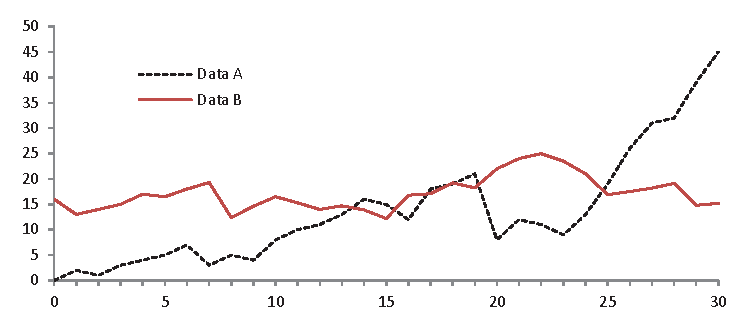
\includegraphics[width=\textwidth]{fig1.eps}
\caption{A figure caption is always placed below the illustration.
Please note that short captions are centered, while long ones are
justified by the macro package automatically.} \label{fig2}
\end{figure}

\begin{theorem}
This is a sample theorem. The run-in heading is set in bold, while
the following text appears in italics. Definitions, lemmas,
propositions, and corollaries are styled the same way.
\end{theorem}
%
% the environments 'definition', 'lemma', 'proposition', 'corollary',
% 'remark', and 'example' are defined in the LLNCS documentclass as well.
%
\begin{proof}
Proofs, examples, and remarks have the initial word in italics,
while the following text appears in normal font.
\end{proof}
For citations of references, we prefer the use of square brackets
and consecutive numbers. Citations using labels or the author/year
convention are also acceptable. The following bibliography provides
a sample reference list with entries for journal
articles~\cite{ref_article1}, an LNCS chapter~\cite{ref_lncs1}, a
book~\cite{ref_book1}, proceedings without editors~\cite{ref_proc1},
and a homepage~\cite{ref_url1}. Multiple citations are grouped
\cite{ref_article1,ref_lncs1,ref_book1},
\cite{ref_article1,ref_book1,ref_proc1,ref_url1}.

%
% ---- Bibliography ----
%
% BibTeX users should specify bibliography style 'splncs04'.
% References will then be sorted and formatted in the correct style.
%
\bibliographystyle{splncs04}
\bibliography{CS3243_project_1}

\begin{thebibliography}{8}
\bibitem{ref_article1}
Author, F.: Article title. Journal \textbf{2}(5), 99--110 (2016)

\bibitem{ref_lncs1}
Author, F., Author, S.: Title of a proceedings paper. In: Editor,
F., Editor, S. (eds.) CONFERENCE 2016, LNCS, vol. 9999, pp. 1--13.
Springer, Heidelberg (2016). \doi{10.10007/1234567890}

\bibitem{ref_book1}
Author, F., Author, S., Author, T.: Book title. 2nd edn. Publisher,
Location (1999)

\bibitem{ref_proc1}
Author, A.-B.: Contribution title. In: 9th International Proceedings
on Proceedings, pp. 1--2. Publisher, Location (2010)

\bibitem{ref_url1}
LNCS Homepage, \url{http://www.springer.com/lncs}. Last accessed 4
Oct 2017
\end{thebibliography}

\appendix
\section{Proof for Manhattan Distance Consistency}
\label{appendix:manhat_cons}

To prove that Manhattan Distance is consistent.
\begin{proof} Proof by Cases
    \begin{enumerate}
        \item \( |h(n') - h(n) = 1| \) (\( \because c(n, a, n') = 1 \), any node n' is 1 step away from node n)
        \item Case 1: \( h(n') = h(n) + 1 \)
        \begin{enumerate}
            \item \( h(n) \leq h(n) + 1 + 1 \implies h(n) \leq h(n') + c(n, a, n') \)
        \end{enumerate}
        \item Case 2: \( h(n') = h(n) - 1 \)
        \begin{enumerate}
            \item \( h(n) \leq h(n) - 1 + 1 \implies h(n) \leq h(n') + c(n, a, n') \)
        \end{enumerate}
        \item For both cases of \( h(n') \), \( h(n) \) is consistent. (\(\bullet\))
    \end{enumerate}
\end{proof}

\end{document}
